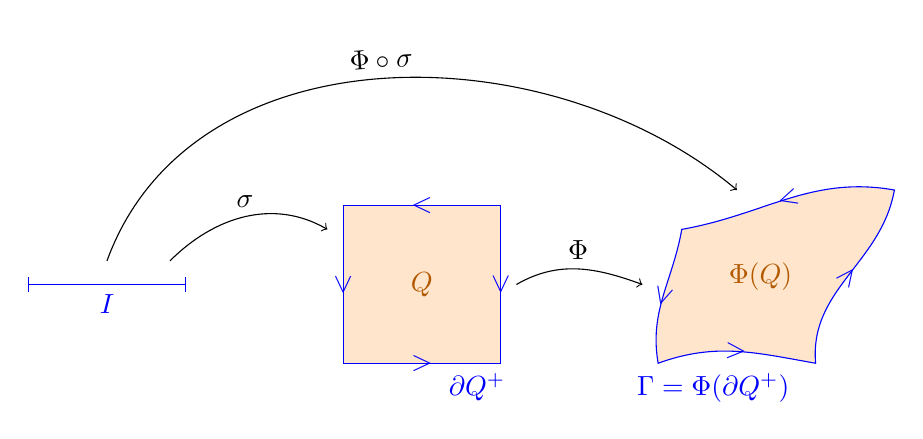
\begin{tikzpicture}
\draw[blue,|-|] (0,0) -- (2,0) node[midway,below] {$I$}; % Intervalo I

\draw[->] (1.8,0.3) to[out=45, in=150] node[midway,above] {$\sigma$} (3.8,0.7) ;

% % Primer cuadrado
\fill[orange!20!white,draw=none] (4,1) rectangle (6,-1);

\draw[blue] (4,-1) -- (4,1) node[midway,sloped] {\textless};
\draw[blue] (4,1) -- (6,1) node[midway,sloped] {\textless};
\draw[blue] (6,1) -- (6,-1) node[midway,sloped] {\textgreater};
\draw[blue] (6,-1) -- (4,-1) node[midway,sloped] {\textgreater};

\node[orange!70!black] at (5,0) {$Q$};
\node[blue,below] at (5.7,-1) {$\partial Q^+$}; 

\draw[blue, fill=orange!20!white] 
	(8,-1) to[out=100, in=260] node[midway,sloped] {\textless} 
	(8.3,0.7) to[out=10, in=170] node[midway,sloped] {\textless} 
	(11,1.2) to[out=260, in=95] node[midway,sloped] {\textgreater} 
	(10,-1) to[out=170, in=20] node[midway,sloped] {\textgreater}  (8,-1) -- cycle;

\draw[->] (6.2,0) to[out=30, in=160] node[midway,above] {$\Phi$} (7.8,0);	

\node[orange!70!black] at (9.3,0.1) {$\Phi(Q)$};
\node[blue,below] at (8.7,-1) {$\Gamma = \Phi(\partial Q^+)$};

\draw[->] (1,0.3) to[out=70, in=140] node[above,sloped] {$\Phi\circ\sigma$} (9,1.2);
\end{tikzpicture}